


\documentclass{article}
\title{Elevator Project UML}
\author{Ridge Rouzier}

\usepackage{pgf-umlcd}
\begin{document}
\maketitle
+ is for public things

	- is for private things
	
	\# is for abstract things


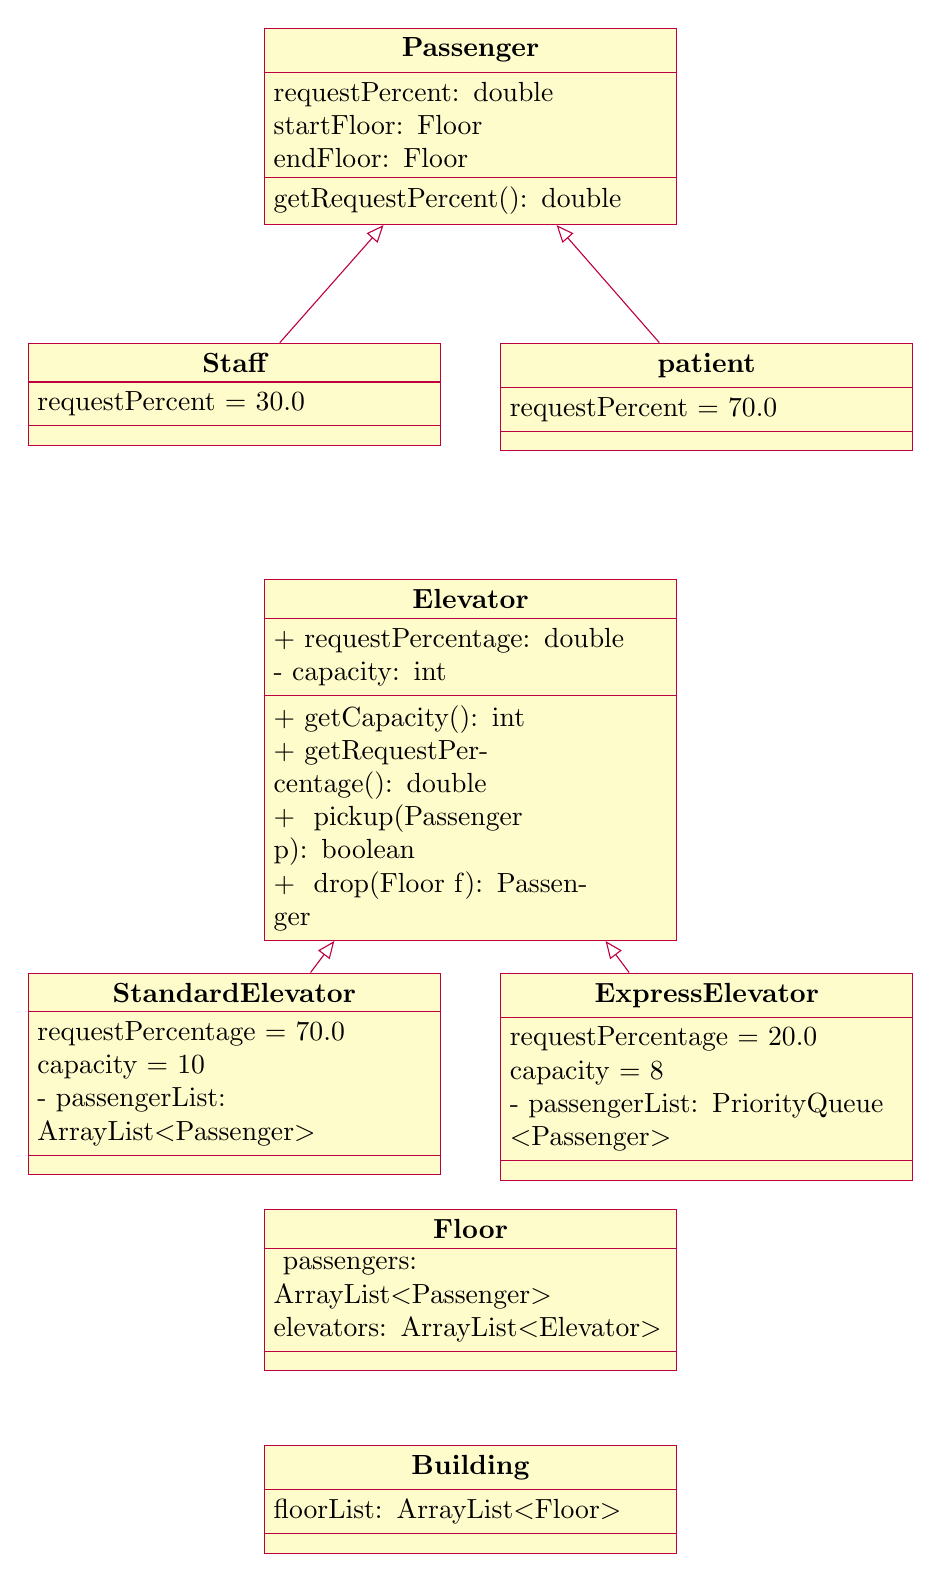
\begin{tikzpicture}
	
	%Passenger class
\begin{class}{Passenger}{0,4}
 \attribute{requestPercent: double}
	\attribute{startFloor: Floor}
	\attribute{endFloor: Floor}
\operation{getRequestPercent(): double}



\end{class}


%patient class
	\begin{class}{patient}{3,0}

\inherit{Passenger}
\attribute{requestPercent = 70.0}

\end{class}

%Staff class
	\begin{class}{Staff}{-3,0}
\inherit{Passenger}

\attribute{requestPercent = 30.0}

\end{class}


	\begin{class}{Elevator}{0,-3}
		\attribute{+ requestPercentage: double}
		\attribute{- capacity: int}
		\operation{+ getCapacity(): int}
		\operation{+ getRequestPercentage(): double}
		\operation{+~ pickup(Passenger p): boolean}
		\operation{+~ drop(Floor f): Passenger}

	\end{class}

	\begin{class}{StandardElevator}{-3,-8}

		\inherit{Elevator}
		\attribute{requestPercentage = 70.0}
		\attribute{capacity = 10}
		\attribute{- passengerList: ArrayList$<$Passenger$>$}
	\end{class}


	\begin{class}{ExpressElevator}{3,-8}
		\inherit{Elevator}
		\attribute{requestPercentage = 20.0}
		\attribute{capacity = 8}
		\attribute{- passengerList: PriorityQueue $<$Passenger$>$}

	\end{class}

	\begin{class}{Floor}{0,-11}
		\attribute{ passengers: ArrayList$<$Passenger$>$}
		\attribute{ elevators: ArrayList$<$Elevator$>$}


	\end{class}


	\begin{class}{Building}{0,-14}
		\attribute{floorList: ArrayList$<$Floor$>$}

	\end{class}

\end{tikzpicture}




\end{document}
